\documentclass[12pt]{article}
\usepackage{amsmath}
\usepackage{amssymb}
\usepackage{tikz}
\begin{document}
\title{Computer Science 181, Homework 1}
\date{April 9th, 2018}
\author{Michael Wu\\UID: 404751542}
\maketitle

\section*{Problem 0}

Each section is assigned a number, starting with zero and increasing by one. Within the text, other elements are numbered in this format
\begin{center}
        Section.Subsection\\
        Section.\{Figure, Example, Theorem\}\\
        Section.\{Exercise, Problem\}\\
\end{center}
The brackets denote that elements belong to the same class and they share a counter, which increases by one. So for example the first
subsection in section \(0\) is numbered \(0.1\), the first figure in section \(0\) is numbered \(0.1\), but the example after that figure
is numbered \(0.2\).

\section*{Problem 1}

\paragraph{a)}

\[\{0^m1^n|m,n\geq0 \wedge m,n\in\mathbb{Z} \}\cup\{1^m0^n|m,n\geq0 \wedge m,n\in\mathbb{Z}\}\]

\paragraph{b)}

\[\{\epsilon,1,0\}\cup\{yxy|x\in\Sigma^* \wedge y\in\Sigma\}\]
Here I use the Kleene star operator. Note that the decision to include \(\epsilon\) is ambiguous based on
how someone interprets the problem statement.

\section*{Problem 2}

\paragraph{a)}

\begin{align*}
\{&(0,000),(0,001),(0,011),(0,111),(0,110),(0,100),\\
&(1,000),(1,001),(1,011),(1,111),(1,110),(1,100)\}
\end{align*}

\paragraph{b)}

\[\{\{0,1\},\{0\},\{1\},\{\}\}\]

\paragraph{c)}

\[|\mathcal{P}(A)|=8\]

\paragraph{d)}

Postponed.

\paragraph{e)}

Postponed.

\paragraph{f)}

\[\{\}\]

\paragraph{g)}

\[\{(\epsilon,a),(\epsilon,b),(\epsilon,c)\}\]

\section*{Problem 3}

First we will prove that a tree that fits the structural definition also fits the recursive definition. If we have a structural rooted tree of height
\(0\) edges, then longest path from the root to any node is of length \(0\) edges. Thus no other nodes can exist in this tree other than the root node, because
if another node was in the tree there would be a path with a length greater than \(0\) edges. Because there are no cycles and only one node, there can be no edges
in a structural rooted tree of height \(0\) edges. Thus we have proven the base case of the recursive definition, that a rooted tree of height \(0\) edges
is a graph with one node and no edges.

Next we must prove that a tree that fits the structural definition with a height of \(n\) edges has at least one rooted subtree of height \(n-1\) edges, and this
subtree's root node is connected by one edge to the root of the tree. We have in the structural definition that the longest path from the root to any node is of length
\(n\) edges. Thus if we take the longest path \(P\), we can create a subtree of height \(n-1\) edge by traveling along \(P\) one node away from the root and letting this
be the root of the subtree. The subtree cannot have a path longer than \(n-1\) edges, because then the parent tree would have a path longer than \(n\) edges, as the subtree
root is one edge away from the parent root. Thus we have proven that each tree of height \(n>0\) edges has a subtree of height \(n-1\) edges whose root is one edge away from
the parent root.

Next we will prove that all the subtrees of a tree that fits the structural definition are not connected to each other. We are given that there are no cycles in a tree
that fits the structural definition. Thus no subtree can be connected to each other, as they are all connected to the root. If two subtrees were connected to each other,
then there would be a cycle because a path would exist from the root to one subtree, then to the second subtree, then back to the root. Thus a tree that fits the structural
definition also fits the recursive definition.

In the reverse direction, we must prove that a tree that fits the recursive definition also fits the structural definition. First we prove that the tree is connected.
Because the recursive definition requires that each subtree be connected to its parent, there cannot be any unconnected parts of the tree. Unless a node is the root of the
tree, there will always be an edge to a parent node. The root of the tree will have one edge to a subtree, unless the height of the tree is \(0\) edges. But a tree of height
\(0\) edges is connected already. So a tree that fits the recursive definition is always connected.

Next we will prove that a tree that fits the recursive definition does not have any cycles. The base case of a height \(0\) edges tree that fits the recursive definition has
no cycles, as there are no edges. For any tree of height \(n>0\) edges, there are no cycles containing the root node. This is because the root node is only connected to subtrees,
and each subtree is disjoint. So traveling from the root node, there cannot be a path that goes from the root node to a subtree, then to another subtree, then back to the root
node. Finally, if each subtree has no cycles, there are no cycles in the entire tree. Since each subtree must have a height of at most \(n-1\) edges, we can use induction to show
that any tree that fits the recursive definition has no cycles. Since the base case has no cycles, and adding a root node does not create a cycle, there can be no cycles at all.

Next we will show that in a tree that fits the recursive definition of height \(n\) edges, every path from the root to another node has at most length \(n\) edges.
Consider the base case of height \(0\) edges. Every path from the root to another node has at most length \(0\) edges, as there are no other nodes. Then given a
tree that fits the recursive definition of height \(n>0\) edges, its longest path will have a length of one more than the length of a subtree of height \(n-1\) edges.
This is because it must have at least one subtree of height \(n-1\) edges, and one edge connects the root of the parent to the subtree. So the longest path in a tree
strictly increases with height, therefore the longest path in any subtree must be the longest path in a subtree with a height of \(n-1\) edges. Thus
the length of the longest path in a tree of height \(n>0\) edges is \(n\). This is due to induction, as the base case has a longest path of \(0\) edges, and when
the height increases by \(1\) the longest path increases by \(1\) edge as well. Therefore any rooted tree that fits the recursive definition also fits the
structural definition, and the recursive definition equals the structural definition.

\section*{Problem 4}

\begin{center}
        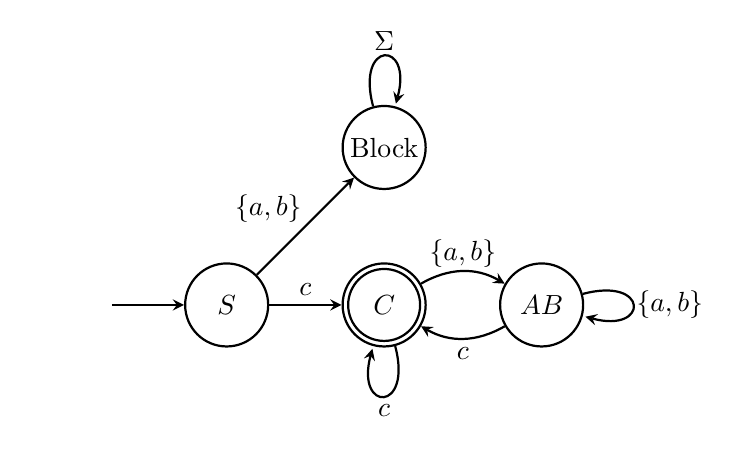
\begin{tikzpicture}
                \begin{scope}[auto, every node/.style={thick, draw,circle,minimum size=3em,inner sep=1}]
                        \node [draw=none] (I) at (-2,0) {};
                        \node (S) at (0,0) {\(S\)};
                        \node (C) at (2,0) {\(C\)};
                        \draw[black, thick] (2,0) circle [radius=1.3em];
                        \node (AB) at (4,0) {\(AB\)};
                        \node (Bl) at (2,2) {Block};
                \end{scope}

                \begin{scope}[auto, every node/.style={minimum size=1em,inner sep=1}, every path/.style={thick, ->, >=stealth}]
                        \path (I) edge (S);
                        \path (S) edge node {\(c\)} (C);
                        \path (S) edge node {\(\{a,b\}\)} (Bl);
                        \path (C) edge [loop below] node {\(c\)} (C);
                        \path (AB) edge [loop right] node {\(\{a,b\}\)} (AB);
                        \path (Bl) edge [loop above] node {\(\Sigma\)} (Bl);
                        \path (C) edge [bend left] node {\(\{a,b\}\)} (AB);
                        \path (AB) edge [bend left] node {\(c\)} (C);
               \end{scope}
        \end{tikzpicture}
\end{center}

\section*{Problem 5}

\begin{center}
        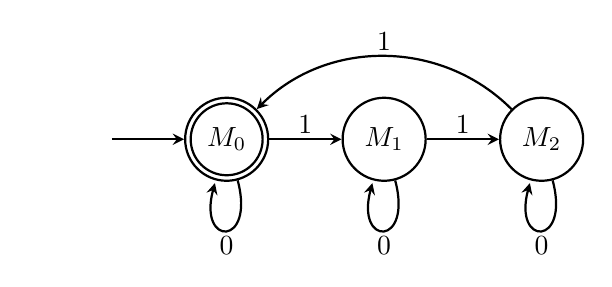
\begin{tikzpicture}
                \begin{scope}[auto, every node/.style={thick, draw,circle,minimum size=3em,inner sep=1}]
                        \node [draw=none] (I) at (-2,0) {};
                        \node (0) at (0,0) {\(M_0\)};
                        \draw[black, thick] (0,0) circle [radius=1.3em];
                        \node (1) at (2,0) {\(M_1\)};
                        \node (2) at (4,0) {\(M_2\)};
                \end{scope}

                \begin{scope}[auto, every node/.style={minimum size=1em,inner sep=1}, every path/.style={thick, ->, >=stealth}]
                        \path (I) edge (0);
                        \path (0) edge node {\(1\)} (1);
                        \path (1) edge node {\(1\)} (2);
                        \path (2) edge [bend right=45] node [above] {\(1\)} (0);
                        \path (0) edge [loop below] node {\(0\)} (0);
                        \path (1) edge [loop below] node {\(0\)} (1);
                        \path (2) edge [loop below] node {\(0\)} (2);
               \end{scope}
        \end{tikzpicture}
\end{center}

\section*{Problem 6}

\paragraph{a)}

This is the set \(S\) of all strings \(s\) in which all contiguous substrings of \(s\) made entirely of \(b\)'s have an odd length,
and all contiguous substrings of \(s\) made entirely of \(a\)'s have an even length.

\paragraph{b)}

This is the set \(S\) of all strings \(s\) over \(\Sigma=\{0,1\}\) which are not made entirely of \(0\)'s, and end in either
\(1\) or an even number of \(0\)'s.

\paragraph{c)}

This is the set \(S\) of all strings \(s\) over \(\Sigma=\{0,1\}\) that end in \(1\).

\end{document}